\documentclass[onecolumn, oneside, letterpaper, draftclsnofoot, 10pt, compsoc]{IEEEtran}

\usepackage{pdfpages}
\usepackage{graphicx}

\usepackage[english]{babel}

\usepackage[hyphens]{url}
\usepackage{setspace}
\usepackage{subcaption}

\usepackage{amssymb}
\usepackage{amsmath}
\usepackage{amsthm}
\usepackage{alltt}
\usepackage{color}
\usepackage{enumitem}
\usepackage{textcomp}
\usepackage{cite}
\usepackage{listings}

\usepackage{lmodern}
\usepackage[hidelinks]{hyperref}
\usepackage[normalem]{ulem}

\usepackage[utf8]{inputenc}
\usepackage[english]{babel}
\usepackage{lineno}
\usepackage{upquote}
\usepackage{fvextra}
\usepackage{fancyvrb}
\usepackage{minted}
\usepackage{longtable,hyperref}

\usepackage[T1]{fontenc}

\usepackage[margin=0.75in]{geometry}

\parindent = 0.0 in
\parskip = 0.0 in

\newcommand{\longtableendfoot}{Please continue at the next page}

% 1. Fill in these details
\def \CapstoneTeamName{         Beaver Hawks}
\def \CapstoneTeamNumber{       14}
\def \GroupMemberOne{           Anton Synytsia}
\def \GroupMemberTwo{           Matthew Phillips}
\def \GroupMemberThree{         Shanmukh Challa}
\def \GroupMemberFour{          Nathan Tan}
\def \CapstoneProjectName{      American Helicopter Society Micro Air Vehicle Competition}
\def \CapstoneSponsorCompany{   Columbia Helicopters}
\def \CapstoneSponsorPerson{    Nancy Squires}

\def \DocType{Requirements Document}

\newcommand{\NameSigPair}[1]{\par
\makebox[2.75in][r]{#1} \hfil   \makebox[3.25in]{\makebox[2.25in]{\hrulefill} \hfill        \makebox[.75in]{\hrulefill}}
\par\vspace{-12pt} \textit{\tiny\noindent
\makebox[2.75in]{} \hfil        \makebox[3.25in]{\makebox[2.25in][r]{Signature} \hfill  \makebox[.75in][r]{Date}}}}
% 3. If the document is not to be signed, uncomment the RENEWcommand below
%\renewcommand{\NameSigPair}[1]{#1}

%%%%%%%%%%%%%%%%%%%%%%%%%%%%%%%%%%%%%%%
\begin{document}
\begin{titlepage}
    \pagenumbering{gobble}
    \begin{singlespace}
        %\includegraphics[height=4cm]{coe_v_spot1}
        \hfill
        % 4. If you have a logo, use this includegraphics command to put it on the coversheet.
        \begin{center}
        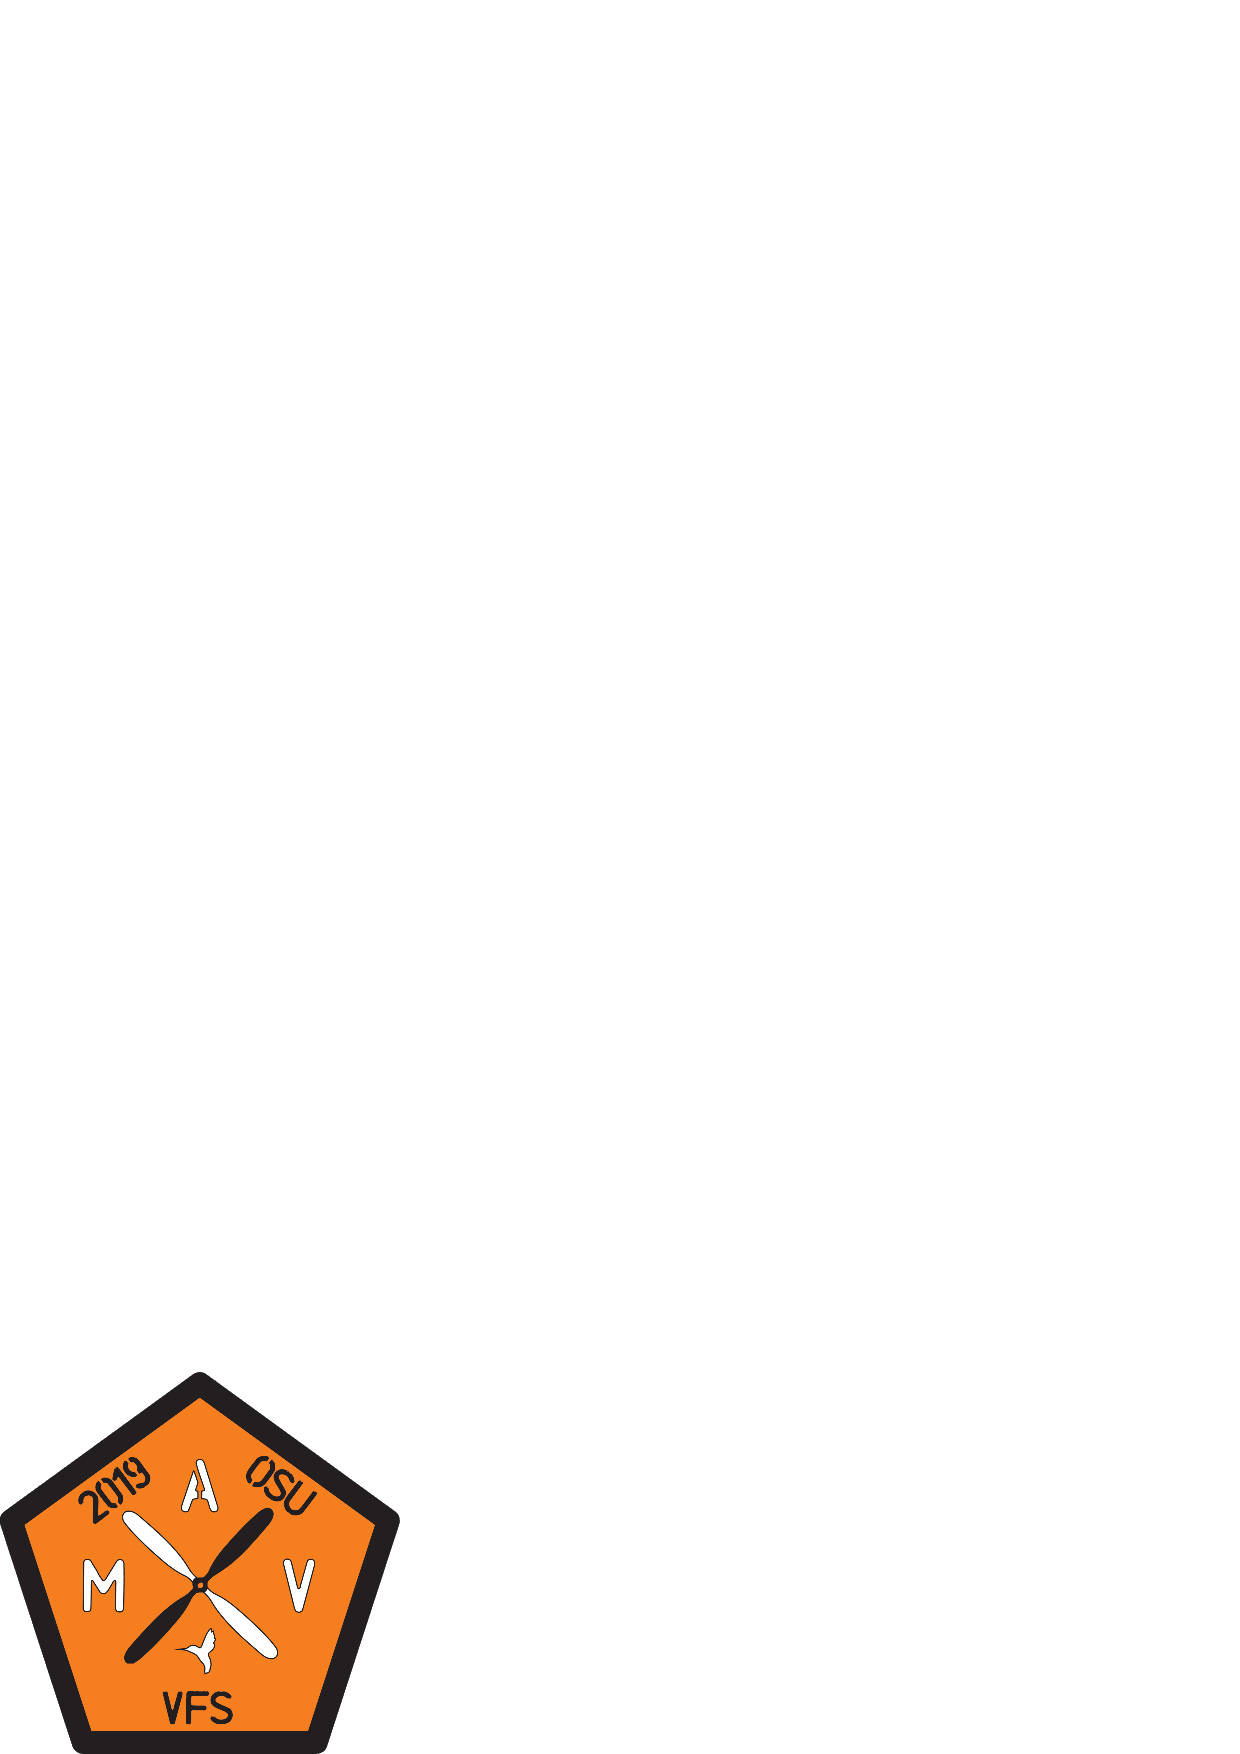
\includegraphics[height=4cm]{graphics/logo.png}
        \end{center}
        \par\vspace{.2in}
        \centering
        \scshape{
            \huge CS Capstone \DocType \par
            {\large\today}\par
            \vspace{.5in}
            \textbf{\Huge\CapstoneProjectName}\par
            \vfill
            {\large Prepared for}\par
            \Huge \CapstoneSponsorCompany\par
            \vspace{5pt}
            {\Large\NameSigPair{\CapstoneSponsorPerson}\par}
            {\large Prepared by }\par
            Group\CapstoneTeamNumber\par
            % 5. comment out the line below this one if you do not wish to name your team
            \CapstoneTeamName\par
            \vspace{5pt}
            {\Large
                \NameSigPair{\GroupMemberOne}\par
                \NameSigPair{\GroupMemberTwo}\par
                \NameSigPair{\GroupMemberThree}\par
                \NameSigPair{\GroupMemberFour}\par
            }
            \vspace{20pt}
        }
        \begin{abstract}
        \noindent
        Oregon State University (OSU) is participating in this year\textquotesingle s Mirco Air Vehicle (MAV) Challenge hosted by the Vertical Flight Society (VFS). The VFS hosts the annual MAV Challenge to attract interest from future scientists and engineers, and to promote vertical flight technology. OSU\textquotesingle s team is comprised of Mechanical Engineers, Electrical and Computer Engineers, and Computer Scientists. This document covers the expected functionality of OSU\textquotesingle s MAV software, developed and written by the team\textquotesingle s Computer Scientists. 
        \end{abstract}
    \end{singlespace}
\end{titlepage}
\newpage
\pagenumbering{arabic}
\tableofcontents
% 7. uncomment this (if applicable). Consider adding a page break.

\listoffigures
%\listoftables
\clearpage

\newpage
\begin{center}
  \begin{tabular}{ | l | p{5cm} | p{5cm} | }
    \hline
    Section & Original & New \\ \hline
    1.3 & Section 1.3 stated that the project will include functionalities such as collision avoidance and autonomous features. However, after considering the aircraft's final functionality, available hardware limitations, and safety factors, we decided against these technologies.  & The updated document removes any reference of these technologies as they were not pursued. \\ \hline
    1.5 & Section 1.5 contained definitions that were relevant to our previously planned product. & The new version removes any references to the features that we did not have the bandwidth to build. \\ \hline
    2.1 & This section referred to hardware that were no longer used. & The new document removes any hardware component that is not being used. \\ \hline
  \end{tabular}
\end{center}
\newpage

\section{Introduction}

\subsection{Purpose}
This document establishes definite project requirements of the Computer Science team\textquotesingle s portion of the Vertical Flight Society\textquotesingle s Micro Air Vehicle obstacle course challenge. Each requirement is described in detail.

\subsection{Scope}
This document is constrained to the CS team’s work on the MAV. The primary focus for our project is to build an aviation user interface to display data feeds from the onboard cameras and sensors. The software is intended for the MAV pilot to use during the competition.

\subsection{Product Overview}
This document covers the interactions between the different features, how users are supposed to interact with the team’s MAV, assumptions made by the team, and the constraints faced by the team.

\subsubsection{Product Perspective}
The MAV will transmit sensor data, which the CS team’s software will capture and process. The software is intended for the pilot to use while flying the aircraft to help create informed flight control decisions. The software displays data feeds from flight sensors including speed, height, vehicle orientation, and two cameras onboard the helicopter. Additionally, the software is built with a scalable framework which allows for new data feeds to be added with ease.

\subsubsection{Product Functions}
The MAV will have a dedicated laptop computer that handles data processing and flight controls. Computer software will process incoming camera and sensory information and provide the pilot with visual feedback.

\subsubsection{User Characteristics}
The MAV is controlled remotely by an experienced pilot. A visual display with camera and sensor data will provide the pilot with additional information to help guide the pilot when the MAV is out of line of sight..

\subsubsection{Limitations}
The competition and the MAV should conform to the rules established by the Vertical Flight Society, which enforce safety considerations, inclusion of remote control functionality, a 500 gram weight limit, a 45 centimeter dimension limit in any direction, and inclusion of an onboard camera. The 500 gram weight limit and budget limitations prevent the use of desired hardware, including an \textit{Eys3D} camera, certain types of range finding sensors, high bandwidth broadcasting equipment, and powerful on-board processing units.

\subsection{Apportioning of Requirements}
Figure \ref{fig:GanttChart} is a Ghantt chart that describes our estimated timeline of completing tasks. Each phase needs to be completed by the end of it’s width. Documents for the grade portion of this project are due by the end of each term, denoted by the green bars. In terms of the CS team, code for the various helicopter components should be feature complete by the end of winter term.
\begin{figure}[h]
    \centering
    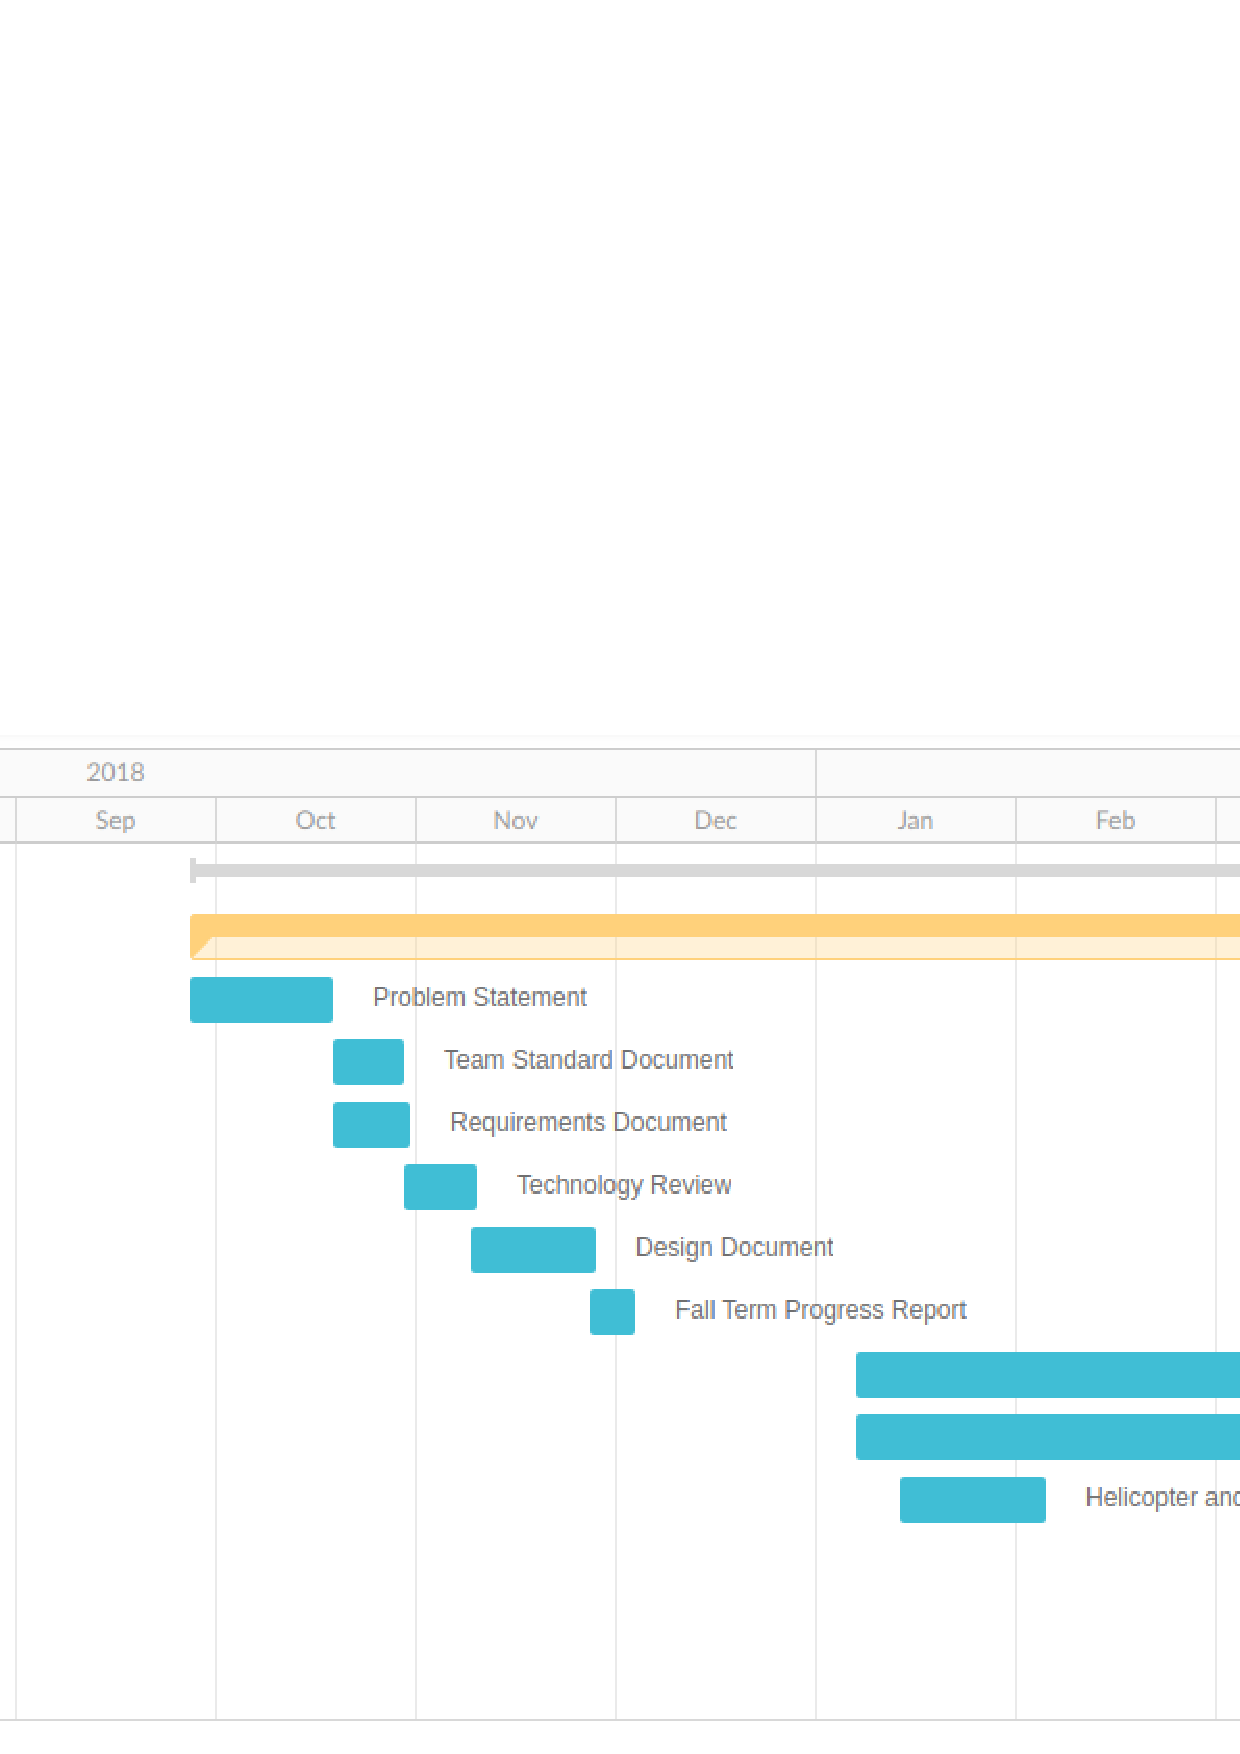
\includegraphics[width=1.0\textwidth]{graphics/gantt_chart.png}
    \caption{Completion Timeline}
    \label{fig:GanttChart}
\end{figure}

\subsection{Definitions}
\begin{itemize}
    \item \textbf{Anti-Torque}: Rotational control of helicopter.
    \item \textbf{Collective}: Pitch angle of helicopter\textquotesingle s main rotor blades.
    \item \textbf{Cyclic}: Pitch and roll (tilt) of a helicopter\textquotesingle s main rotor.
    \item \textbf{GUI}: Graphical user interface.
    \item \textbf{Micro Air Vehicle (MAV)}: A remotely controlled, semi-autonomous, coaxial helicopter.
    \item \textbf{OSU}: Oregon State University.
    \item \textbf{Package}: A sealed paper lunch bag, containing a pamphlet, shown in figure \ref{fig:Bag}. A braided wire loop is attached at the top of the bag for acquirement.
    \item \textbf{Package A}: A package weighing between 20 and 25 grams.
    \item \textbf{Package B}: A package weighing between 25 and 30 grams.
    \item \textbf{Throttle}: Engine power to helicopter\textquotesingle s main rotor.
    \item \textbf{VFS}: Vertical Flight Society.
\end{itemize}
\begin{figure}[h]
    \centering
    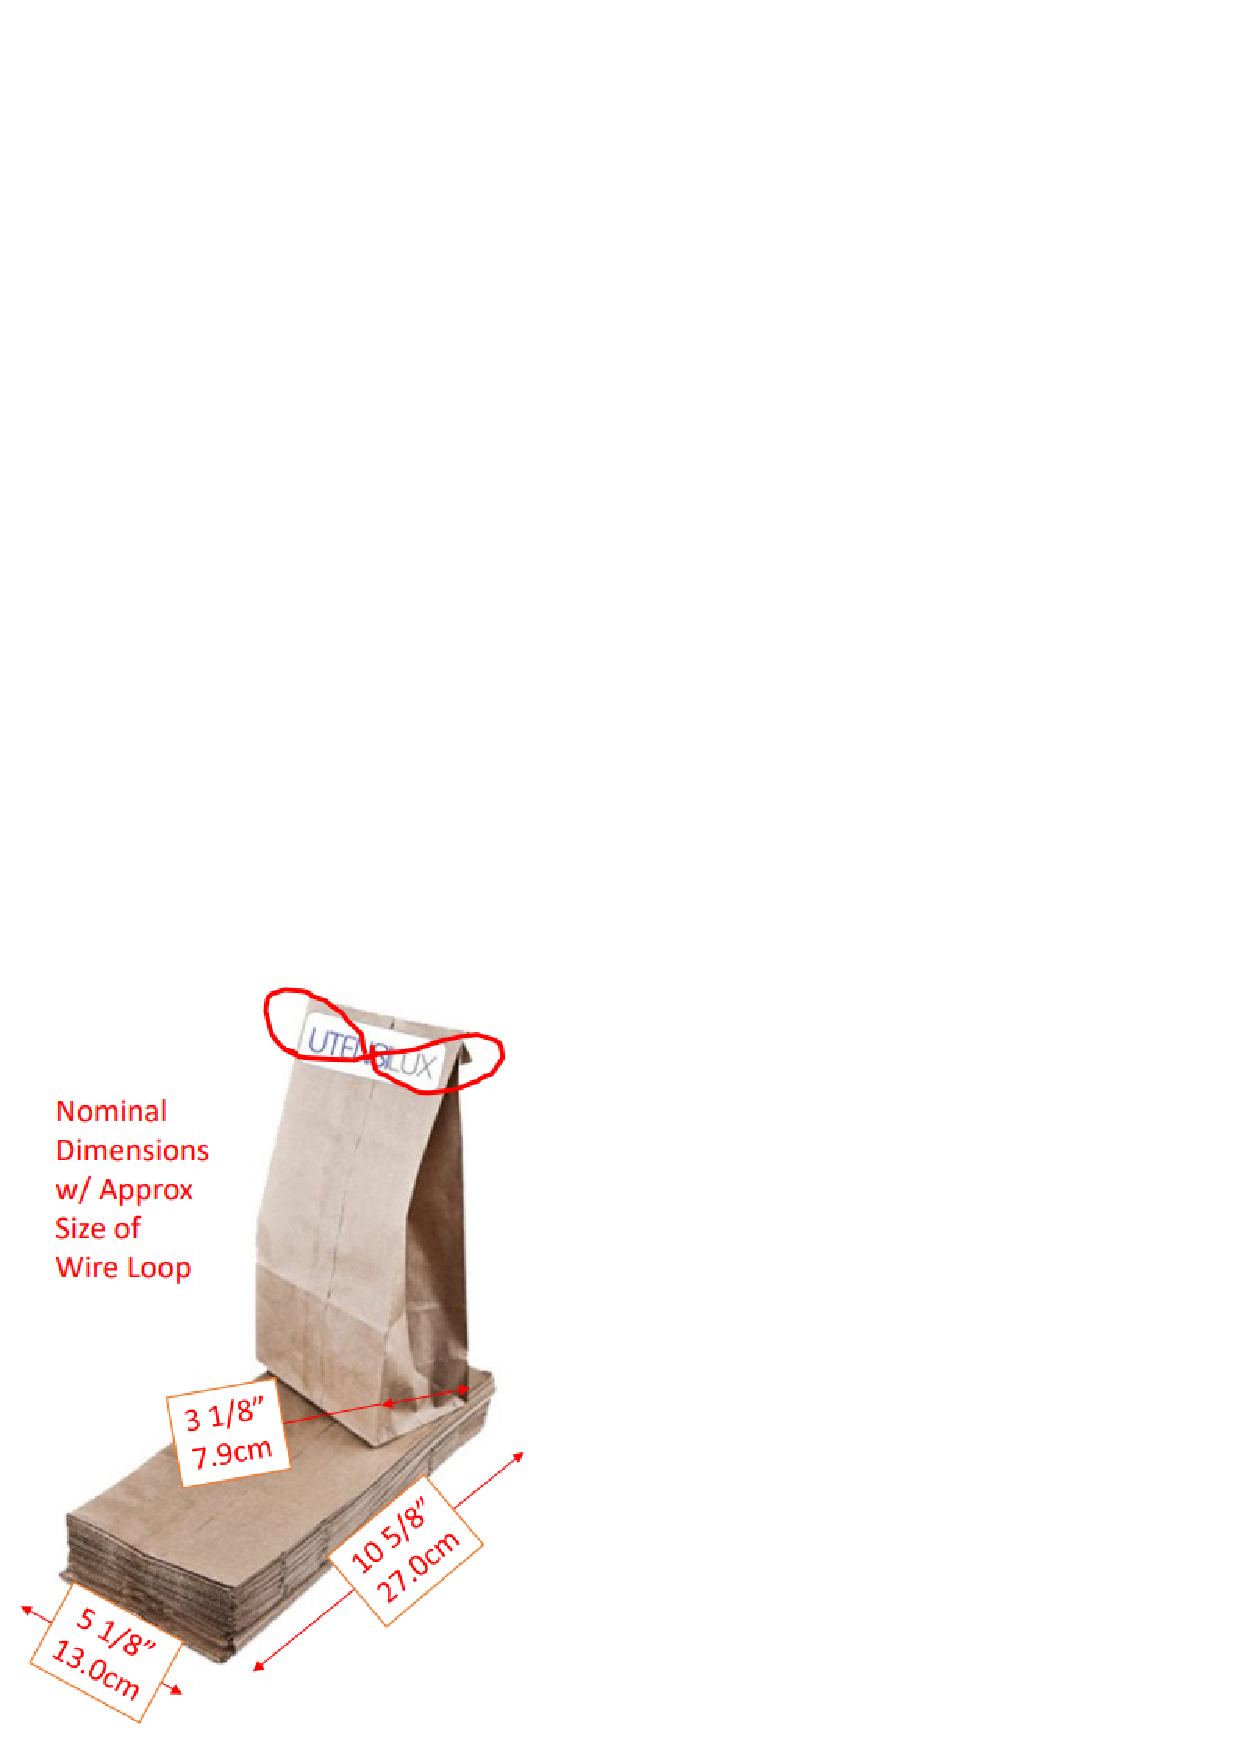
\includegraphics[height=4cm]{graphics/bag.png}
    \caption{Package}
    \label{fig:Bag}
\end{figure}

\subsection{References}
[1]
\newblock Vertical Flight Society. (2018).
\newblock {\em 7th Annual VFS Micro Air Vehicle (MAV) Student Challenge} [PDF file].
\newblock Retrieved from \url{https://vtol.org/files/dmfile/7th-annual-mav-student-challenge_v7_oct182018.pdf?fbclid=IwAR3-J_yJIKUKoGPBfsdJ}\\ \url{FAbjMUzXoxwg1hCXiQi6JnWZRLOnSMBRnMmQGKU}.

[2]
\newblock Standford CS-231. (2018).
\newblock {\em Convolutional Neural Networks for Visual Recognition}.
\newblock Retrieved from \url{http://cs231n.github.io/convolutional-networks/}.

[3]
\newblock Federal Aviation Administration. (2018).
\newblock {\em Helicopter Flying Handbook}.
\newblock Retrieved from \url{https://www.faa.gov/regulations_policies/handbooks_manuals/aviation/helicopter_flying_handbook/media/hfh_ch03.pdf}.

\section{Specific Requirements}
This section contains all the input and functional requirements of the MAV\textquotesingle s software.

\subsection{External Interfaces}
The following section composes hardware components required for the software.

\noindent
\textbf{Tool ID: FC}\\
Name: Flight Controls\\
Description: Controls for adjusting cyclic, collective, anti-torque, and throttle.\\
Inputs: GRYO, ACCL, MRTRAN\\
Output: MRTRAN\\

\noindent
\textbf{Tool ID: GYRO}\\
Name: Gyroscope\\
Description: A gyroscope is needed to stabilize all three axes of alignment of the coaxial helicopter. The device will prevent the aircraft from flipping over and provide orientation data for flight controls.\\
Output destination: MRTRAN\\

\noindent
\textbf{Tool ID: ACCL}\\
Name: Accelerometer\\
Description: To keep the helicopter stable, there is a need for small reading changes in the motion of the helicopter. The addition of the accelerometer data will significantly improve the helicopter’s ability to maintain a stable position.\\
Output destination: MRTRAN\\

\noindent
\textbf{Tool ID: NCAM}\\
Name: Nose Camera\\
Description: Front facing color camera to provide the pilot with flight visuals.\\
Output destination: MRTRAN\\

\noindent
\textbf{Tool ID: ACAM}\\
Name: Acquire Camera\\
Description: Downward facing color camera to provide the pilot with flight visuals.\\
Output destination: MRTRAN\\

\noindent
\textbf{Tool ID: MRTRAN}\\
Name: MAV’s Radio Transmitter/Receiver\\
Description: The onboard transmitter will broadcast the MAV sensor data to the receiver connected to the team’s dedicated computer and receive flight control data.\\
Inputs: GRYO, ACCL, IRL, IRCAM, NCAM, ACAM, IRRANG, URANG, CRTRAN, FC\\
Output destination: CRTRAN, FC\\

\noindent
\textbf{Tool ID: CRTRAN}\\
Name: Computer Radio Transmitter/Receiver\\
Description: The radio transmitter/receiver connect to the pilot’s computer for communication with the MAV.\\
Input: MRTRAN\\
Output: MRTRAN, DPROC\\

\noindent
\textbf{Tool ID: DPROC}\\
Name: Processing Unit\\
Description: A dedicated, standalone computer for processing incoming camera and sensor data. Also responsible for processing commands for the MAV. Includes physical display.\\
Input: CRTRAN\\
Output: CRTRAN

\subsection{Functions}
The following section composes hardware software functionalities.\\

\noindent
\textbf{Feature ID: VDISP}\\
Name: Visual Display\\
Description: Outputs a user interface that displays sensor data.\\
Dependencies: None\\
Input: DPROC\\

\subsection{Competition Walkthrough}
The MAV must complete an obstacle course mission themed as Washington\textquotesingle s Flight for Liberty. Figure \ref{fig:CourseMap} displays a mock-up of an obstacle course. Step-by-step objectives of an obstacle course are as follows:
\begin{enumerate}
\item The mission begins with the MAV parked at Thomas Paine’s helipad. Upon the start of a ten minute timer, the MAV must do the following:
\begin{enumerate}
\item Take off from the helipad.
\item Hover for ten seconds.
\item Acquire Package A.
\item Hover for ten seconds.
\item Fly North until reached the net barrier.
\end{enumerate}
\item Upon reaching the the barrier, the pilot must:
\begin{enumerate}
\item Climb MAV 1.83 meters, plus a safe height, above the barrier.
\item Spot and verbally express visual contact with McKonkey’s Ferry.
\item Fly north, descending to a safe height, until reached and passed the center line of McKonkey’s Ferry, by approximately 0.5 meters.
\end{enumerate}
\item Once within 0.91 meters from the northern side of McKonkey’s Ferry, the MAV must head east, until crossed Delaware River and reached Pamphlet Delivery helipad.
\item At Pamphlet Delivery helipad, the MAV must release the package, as close to the bullseye as possible.
\item After releasing the package, the pilot must maneuver MAV south, to Camp Washington Pickup Zone. On its way, the MAV must:
\begin{enumerate}
\item Fly over a 1.22 meter high barrier.
\item Fly under a 0.61 meter obstacle.
\end{enumerate}
\item At the Camp Washington Pickup Zone, the MAV must:
\begin{enumerate}
\item Acquire Package B.
\item Hover for ten seconds.
\item Head back to Thomas Paine’s helipad, reversing the route.
\end{enumerate}
\item Upon reaching Thomas Paine’s helipad, the pilot must:
\begin{enumerate}
\item Verbally express visual contact with Thomas Paine’s helipad.
\item Have the MAV release the package as close to the bullseye as possible.
\item Land the MAV within 0.91 meters of the helipad.
\end{enumerate}
\end{enumerate}
\begin{figure}[h]
    \centering
    \includegraphics[width=0.5\textwidth]{graphics/course_map.png}
    \caption{Course Map}
    \label{fig:CourseMap}
\end{figure}

\subsection{Verification}
Measurement is done by the qualitative assessment of mission phases described below:
\begin{description}
\item[Take off and Hover] The MAV must perform a stable hover, above base, at a height of two meters.
\item[En Route to Delivery/Pickup Area] The MAV must have a clearly-announced, timed, and smooth transition to the package delivery and package pick up sites.
\item[Obstacle Avoidance]The MAV must avoid obstacles between the home base the target search area. Metrics include successful avoidance and smoothness of flight around obstacles.
\item[Target Acquisition] The MAV must establish a stable hover for at least five seconds over each delivery/pickup location target and smoothly transition between searching, hover, and drop-off/pickup phases. Metrics include lateral target tracking error and stable roll/pitch performance.
\item[En Route Return to Base] The MAV must return to base with a user signal. Remote operator can use LOS. "Base" can use homing beacons for autonomous return to base. Metrics include qualitative smoothness of transitions and time to acquire stable hover over base.
\item[Hover and Landing] The MAV must acquire a stable hover, two meters above base, before landing. Metrics include hover and landing performance, as well as, distance from the center of the helipad.
\end{description}

\end{document}
